% Figure 6 of "The architecture of blockchain value: capabilities, pillars, and growth dynamics"
% (Papadogiannis, 2026, Front. Blockchain 9:1747512). Drawing code as in the author's manuscript.
% Compile with: pdflatex fig6_consensus_evolution.tex
\documentclass[border=6pt]{standalone}
\usepackage{amsmath, amssymb}
\usepackage{tikz}
\usetikzlibrary{positioning, shapes, arrows.meta, calc, backgrounds}
\begin{document}
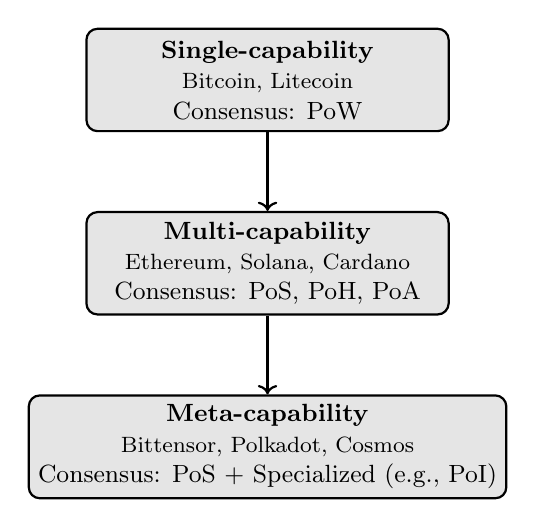
\begin{tikzpicture}[
  node/.style={rectangle, rounded corners, draw=black, thick, align=center, minimum width=4.6cm, minimum height=1.3cm, font=\small, fill=gray!10},
  level distance=1.8cm
]

\node[node, fill=gray!20] (single) {\textbf{Single-capability} \\ \footnotesize Bitcoin, Litecoin \\ Consensus: PoW};
\node[node, below=of single, fill=gray!20] (multi) {\textbf{Multi-capability} \\ \footnotesize Ethereum, Solana, Cardano \\ Consensus: PoS, PoH, PoA};
\node[node, below=of multi, fill=gray!20] (meta) {\textbf{Meta-capability} \\ \footnotesize Bittensor, Polkadot, Cosmos \\ Consensus: PoS + Specialized (e.g., PoI)};

\draw[->, thick] (single.south) -- (multi.north);
\draw[->, thick] (multi.south) -- (meta.north);

\end{tikzpicture}
\end{document}
